\section{Data Centres}\label{sec:cloud:data_centers}
Data centres are used to host most of the applications running in the Internet, including those discussed earlier in this work.
Servers are operated by the data centre operator and rented out to customers as part of a \gls{PaaS} or \gls{IaaS} scheme.
In order to increase revenue the data centre operator is interested in decreasing server power drain, one of the major matters of expense for data centres \cite{Greenberg2009b}, while satisfying \glspl{SLA} with their customers.

This section studies this scenario and provides a model intended for data centre operators to manage this tradeoff.
In \refsec{sec:cloud:data_centers:problem_formulation} we provide a mathematical formulation for the considered scenario.
Then, in \refsec{sec:cloud:data_centers:modeling} we model this scenario using methods from queueing theory and derive metrics which can be used to evaluate the different approaches and configurations of data centres.
In \refsec{sec:cloud:data_centers:closed_form_solution} we present different methods for solving the previously introduced queueing model.
Finally, in \refsec{sec:cloud:data_centers:performance_evaluation} we study the performance implications of the model and discuss the tradeoff between power drain and suffered waiting time.

\subsection{Considered Data Centre Architectures}\label{sec:cloud:data_centers:problem_formulation}

A widely used data centre architecture is the three-tier architecture shown in \reffig{fig:cloud:data_centers:problem_formulation:3-tier_datacenter}.
The upper two layers of the architecture are responsible for distributing the traffic and consist of layer 3 switches where each switch has a backup switch.
In this section, we focus on the edge layer and especially on a single \gls{POD}.
A \gls{POD} consists of a number of servers connected over top of rack switches to an aggregation switch.

\begin{figure}
  \centering
  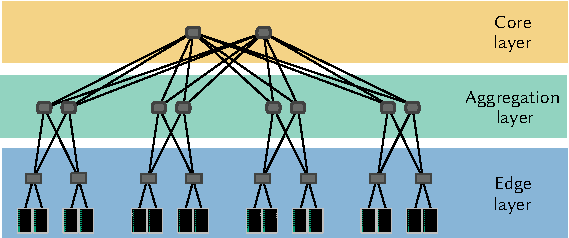
\includegraphics{cloud/data_centers/problem_formulation/figures/architecture}
  \caption{Considered standard three-tier data centre architecture.}
  \label{fig:cloud:data_centers:problem_formulation:3-tier_datacenter}
\end{figure}

We assume that new jobs entering the system arrive with exponentially distributed inter-arrival time.
When a job arrives at the \gls{POD}, it is forwarded to an idle server.
If no idle server is available, the job is queued.
Once a server finishes processing its current job, it picks another one from the queue.

Our goal is to evaluate how much power is consumed in a data centre and how much can be saved when servers, currently not processing any job, are switched off.
Therefore, we developed two different data centre models.
The first model, the \emph{traditional data centre}, consists of two-state servers only which are either \emph{busy} or \emph{idle}, as shown in \reffig{fig:cloud:data_centers:problem_formulation:servers:idle_busy} 
For the second model, a more \emph{energy-efficient data centre}, a subset of the servers may additionally be switched \emph{on} and \emph{off} on demand, shown in \reffig{fig:cloud:data_centers:problem_formulation:idle_busy_off} as recommended in~\cite{EPA2007}.

\begin{figure}
	\begin{subfigure}[b]{\textwidth}
	\centering
	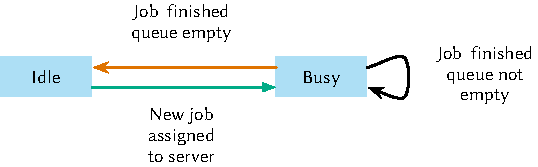
\includegraphics{cloud/data_centers/problem_formulation/figures/idle_busy}
	\caption{2-state server model}\label{fig:cloud:data_centers:problem_formulation:servers:idle_busy}
	\end{subfigure} 
	\begin{subfigure}[b]{\textwidth}
	\centering
	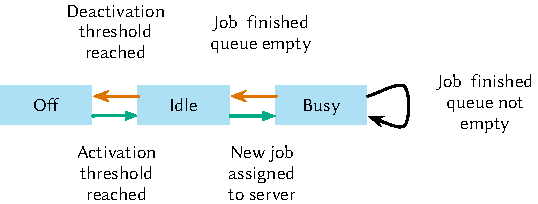
\includegraphics{cloud/data_centers/problem_formulation/figures/idle_busy_off}
	\caption{3-state model of a reserved server}\label{fig:cloud:data_centers:problem_formulation:idle_busy_off}
	\end{subfigure}

	\caption{Assumed power state transition on a per server level.}\label{fig:cloud:data_centers:problem_formulation:servers}
\end{figure}

\subsubsection*{Traditional Data Centre}\label{sec:cloud:data_centers:problem_formulation:default_data_center}
For the traditional data centre model, each of the \(n\) servers is either on and processing a job or on and idle as depicted in \reffig{fig:cloud:data_centers:problem_formulation:servers:idle_busy}.
If a busy server finishes processing a job and the queue is empty, the server becomes idle. Once a new job is assigned to a yet idle server, the server becomes busy.
According to our measurements of a server with an Intel twelve core processor \SI{2.67}{\giga\hertz} and \SI{32}{\giga\byte} RAM, a server currently processing a job consumes \(e_{\text{busy}} = \SI{240}{\watt}\).
An idle server still consumes \(e_{\text{idle}} = \SI{170}{\watt}\).

\subsubsection*{Energy-Efficient Data Centre}\label{sec:cloud:data_centers:problem_formulation:energy_efficient_data_center}
For the second model, we differentiate between two types of servers:
\(n\) base-line servers which are always on and \(m\) reserved servers to be enabled on demand.
If they are enabled, their power drain is similar to that of the default data centre model.
If they are disabled, each server consumes \(e_\text{off} = \SI{0}{\watt}\).
The \(n\) servers which are always enabled consume the same power as in the default data centre model.
If the system queue has a length exceeding \(\theta_2\) where \(\theta_2 \in (0, m)\) holds, the \(m\) reserved servers are enabled and stay enabled until the total number of jobs in the system drops to \(\theta_1\) for \(\theta_1 \in (0, n)\).
The transition between power levels for each of the reserved servers is depicted in \reffig{fig:cloud:data_centers:problem_formulation:idle_busy_off}.

The energy-efficient data centre operation model with the parameters \(\theta_1\) and \(\theta_2\) is depicted in \reffig{fig:cloud:data_centers:problem_formulation:model} and described in detail in the next section.

\begin{figure}
  \centering
  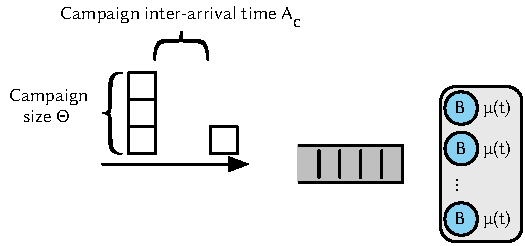
\includegraphics{cloud/data_centers/problem_formulation/figures/model}
  \caption{Considered system model for an energy-efficient data centre.}
  \label{fig:cloud:data_centers:problem_formulation:model}
\end{figure}
\subsection{Model for Energy-Efficient Data Centres}\label{sec:cloud:data_centers:modeling}
In this section, we first discuss the default data centre model, where a server can either be idle or busy, processing a job. Afterwards, the energy-efficient data centre model with three states, i.e. idle, busy, or off, is defined.

\subsubsection*{Traditional Data Centre}\label{sec:cloud:data_centers:modeling:default}
We consider new jobs arriving at a \gls{POD} with exponential \gls{IID} inter-arrival times with rate \(\lambda\).
Each server accepts only one job at a time and processes it with an exponentially distributed service time with mean \(\frac{1}{\mu}\).
Then, the system can be modelled using a simple \(M/M/n\) delay system.
Here, the random variable \(X\) gives the number of jobs in the system and \(x(i)\) is the stationary state probability that \(i\) jobs are currently in the system.

We obtain the mean power drain of such a system based on the measured values presented in \refsec{sec:cloud:data_centers:problem_formulation}.
If less than \(i < n\) jobs are currently in the system, then \(i\) servers are busy each consuming \(e_\text{busy}\) \si{\watt} and \(n-i\) servers are idle, where each consumes \(e_\text{idle}\) \si{\watt}.
If \(i \geq n\) jobs are in the system all servers are busy and consume \(n\cdot e_\text{busy}\) \si{\watt} in total.

For stationary state probabilities \(x(i)\), we obtain the mean power drain as
\begin{equation}\label{sec:cloud:data_centers:modeling:default:emax}
E_\text{max} = \sum_{i=0}^{n} x(i) (i e_\text{busy} + (n-i) e_\text{idle}) + ne_\text{busy} \sum_{i=n + 1}^{+ \infty} x(i).
\end{equation}

Furthermore, we can provide a lower bound for the power drain of the system by assuming that a server is turned off if it is not processing a job, thus consuming \(e_\text{off}\).
By substituting \(e_\text{off}\) for \(e_\text{idle}\) in \refeq{sec:cloud:data_centers:modeling:default:emax} we obtain
\begin{equation*}
E_\text{min} = \sum_{i=0}^{n} x(i) (i e_\text{busy} + (n-i) e_\text{off}) + ne_\text{busy} \sum_{i=n + 1}^{+ \infty} x(i).
\end{equation*}

\subsubsection*{Energy Efficient Data Centre}\label{sec:cloud:data_centers:modeling:energy_efficient}

We extend the queuing system to model the energy-efficient data centre model introduced in \refsec{sec:cloud:data_centers:problem_formulation}, by adapting the state space of the model.
We now model the system state as a tuple \((i,j)\) where \(i\) is gives the number of jobs in the system and \(j\) is \(1\) if the reserved servers are active and \(0\) if they are not.

\begin{figure}[H]
  \centering
  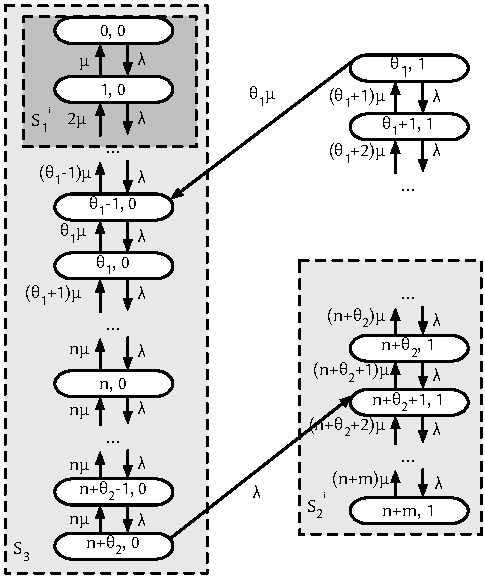
\includegraphics{cloud/data_centers/modeling/figures/state_diagram}
  \caption{\(M/M/(n+m)^{(\theta_1, \theta_2)}\) system with macro states \(S_1^i, S_2^i,\) and \(S_3\) for the calculation of \(x(i, \left\{0, 1\right\})\) in the energy-efficient data centre.}
  \label{fig:cloud:data_centers:modeling:energy_efficient:state_diagram}
\end{figure}

The state diagram for this queueing model is given in \reffig{fig:cloud:data_centers:modeling:energy_efficient:state_diagram}.
The system activates the reserved servers if more than \(\theta_2\) jobs are in the queue, i.e. more than \(n + \theta_2\) jobs are in the system.
The reserved servers are deactivated if the number of jobs in the system drops below \(\theta_1\).

Again, \(X\) is the random variable describing the number of jobs in the system if the reserved servers are activated or deactivated, and \(x(i, j)\) is the stationary probability that \(i\) jobs are in the system, and the reserved servers are activated, for \(j=1\), or deactivated, for \(j=0\). 

Based on the state space and transitions, we formulate macro state equations, defined as the sum of all local balance equations of the states contained in the macro state.
They provide, when solved, the state probabilities required for further analysis. 

First,  we consider the macro state equations for state \(S_1^i\), c.f. \reffig{fig:cloud:data_centers:modeling:energy_efficient:state_diagram}, which contains all system states where up to \(i-1\) jobs are in the system and no reserved servers are activated.
Depending on \(i\), we obtain the following equations
\begin{align}
i\mu x(i,0) &= \lambda x(i-1, 0) & 0<i<\theta_1,\label{eq:cloud:data_centers:modeling:energy_efficient:S1_1}\\
i\mu x(i,0) + \theta_1 \mu x(\theta_1,1) &= \lambda x(i-1,0) & \theta_1\leq i\leq n,\label{eq:cloud:data_centers:modeling:energy_efficient:S1_2}\\
n\mu x(i,0) + \theta_1 \mu x(\theta_1,1) &= \lambda x(i-1,0) & n\leq i\leq n+\theta_2.\label{eq:cloud:data_centers:modeling:energy_efficient:S1_3}
\end{align}

Next, we examine the system state if the reserved servers are activated.
The macro state \(S_2^i\) contains all system states with activated reserved servers and at least \(i+1\) jobs in the system.

We get
\begin{align}
i\mu x(i,1) = \lambda x(i-1,1)\nonumber\\
 + \lambda x(n+\theta_2,0) && \theta_1<i\leq n+\theta_2+1,\label{eq:cloud:data_centers:modeling:energy_efficient:S2_1}\\
 i\mu x(i,1) = \lambda  x(i-1,1) && n+\theta_2+1<i\leq n+m,\label{eq:cloud:data_centers:modeling:energy_efficient:S2_2}\\
 (n+m)\mu x(i,1) =\lambda x(i-1,1) && n+m<i.\label{eq:cloud:data_centers:modeling:energy_efficient:S2_3}
\end{align}

The third macro state \(S_3\) contains all system states where only the base-line servers are activated and its equation states
\begin{equation}
\lambda x(n+\theta_2,0) = \theta_1\mu x(\theta_1,1)\label{eq:cloud:data_centers:modeling:energy_efficient:S3}.
\end{equation}

Finally, the normalisation condition holds:
\begin{equation}
1=\sum_{i=0}^{n+\theta_2} x(i,0)+\sum_{i=\theta_1}^{+\infty}x(i,1).\label{eq:cloud:data_centers:modeling:normative}
\end{equation}

Based on the state probabilities we can derive the required performance metrics for our analysis.

The carried traffic and utilisation is given by
\begin{equation*}
a = \frac{\lambda}{\mu} \text{\quad and\quad} \rho=\frac{\lambda}{\mu(n+m)}.
\end{equation*}

Furthermore, we obtain the mean queue length
\begin{equation*}
\Omega = \sum_{i=n}^{n+\theta_2} (i-n)x(i,0) + \sum_{i=n+m}^{+\infty} (i-(n+m))x(i,1).
\end{equation*}
By applying macro state \refeq{eq:cloud:data_centers:modeling:energy_efficient:S2_3} we obtain for all \(i>n+m\)
\begin{equation}
x(i,1) = \rho x(i-1,1) = x(n + m,1)\rho^{i-(n+m)},
\label{eq:cloud:data_centers:modeling:x_i_redefinition}
\end{equation} 

Using this result and the first derivative of the geometric series we get 
\begin{eqnarray*}
\Omega &=& \sum_{i=n}^{n+\theta_2} (i-n)x(i,0) + x(n+m,1)\sum_{i=0}^{+\infty} i\rho^i\nonumber\\
&=& \sum_{i=n}^{n+\theta_2} (i-n)x(i,0) + x(n+m,1)\frac{\rho}{(1-\rho)^2}.
\end{eqnarray*}

Now, we can give the mean waiting time for all jobs in the system as
\begin{equation*}
E[W] = \frac{\Omega}{\lambda}.
\end{equation*}
Finally, we obtain the mean power drain similarly to \refeq{sec:cloud:data_centers:modeling:default:emax} as
\begin{align*}
E& = \sum_{i=0}^{n} x(i,0)(i e_\text{busy} + (n-i)e_\text{idle} + m e_\text{off})\\
&+ \sum_{i=n+1}^{n+\theta_2} x(i,0)(ne_\text{busy}+me_\text{off})\nonumber\\
&+\sum_{i=\theta_1}^{n+m} x(i,1)(i e_\text{busy} + (n+m-i)e_\text{idle})\nonumber\\
&+x(i > n+m)(n+m)e_\text{busy}.\nonumber
\end{align*}

\subsection{Analysis of Proposed Data Centre Models}\label{sec:cloud:data_centers:closed_form_solution}
Using the macro state equations discussed in \refsec{sec:cloud:data_centers:modeling}, there are multiple ways to obtain the state probabilities.
This section examines the different approaches.

\subsubsection*{System of Linear Equations}
First, it is possible to directly solve the system of linear equations implied by the micro or macro states.
Solvers for linear equation systems scale cubic in the dimension of the matrix, which in this case is bounded by the system size.
Especially for a large numbers of server, this prevents an exhaustive search of the parameter space.

\subsubsection*{Closed-form Solutions}
Thus, we obtain closed form solutions for the state probabilities.
These equations can be derived by recursively applying the macro state equations.

All equations feature a factor \(x(0, 0)\) which in turn can be calculated using the normalisation property given in \refeq{eq:cloud:data_centers:modeling:normative}.
Due to the length of the individual formulas, the following shorthand is introduced:
For each state probability \(x(i, j)\) depending on the factor \(x(0,0)\) we define \(\bar{x}(i, j) = x(i, j) \cdot x(0, 0)^{-1}\), i.e. we cancel the factor.

For \(0 < i <\theta_1\), we get
\begin{align*}
x(i, 0) &= x(0, 0) \cdot \frac{a^i}{i!}.
\end{align*}
As a further shorthand for substitution, we define
\begin{align*}
s_i&=\sum_{k=0}^{i}a^k(n-k-1)!.
\end{align*}
Using this definition, we get the state probability for \(\theta_1\) jobs in the system with activated reserved servers as
\begin{align*}
x(\theta_1, 1) &= x(0, 0)\cdot \frac{a^{n+\theta_2+1}}{\left(1+\frac{a}{\theta_1}\right)}
\cdot\frac{\left(\theta_1-1\right)!\left(\frac{(1-a^{\theta_2})\theta_1}{1-a}+a^{\theta_2}s_{n-\theta_1}\right)}{n^{\theta_2}n!\left(n-\theta_1+1\right)!}.
\end{align*}
For \(\theta_1\leq i\leq n\), we get
\begin{align*}
x(i, 0) = x(0, 0) &\cdot \left(\frac{\bar{x}(n, 0) a^{i-\theta_1+1}}{(i-\theta_1+1)!} - \frac{\bar{x}(\theta_1,1) \theta_1 s_{i-\theta_1}}{i!}\right).
\end{align*}
And for \(n<i\leq n+\theta_2\), we get
\begin{align*}
x(i, 0) = x(0, 0) &\cdot \left(\frac{\bar{x}(n,0) a^{i-\theta_1+1}}{n^{i-n}(n-\theta_1+1)!}\right.\\
&\left.-\bar{x}(\theta_1,1)\left(\frac{\theta_1 s_{n-\theta_1} a^{i-n}}{n!} + \frac{\theta_1(1-a^{i-n})}{1-a}\right)\right).
\end{align*}

Thus, we have all probabilities for system states where only the baseline servers are active. For the reserved servers, we obtain state probabilities for \(\theta_1<i\leq n+\theta_2+1\) as
\begin{align*}
x(i, 1) = x(0, 0) \cdot \left(\bar{x}(\theta_1, 1)\frac{a^{i-\theta_1}\theta_1!}{i!} + \bar{x}(n+\theta_2,0)\sum_{k=1}^{i-\theta_1}\frac{a^k(i-k)!}{i!}\right).
\end{align*}

For \(n+\theta_2+1 < i \leq n + m\), we get
\begin{align*}
x(i, 1) = x(0, 0)\cdot \bar{x}(n+\theta_2+1,1) \cdot\frac{a^{i-(n+\theta_2+1)}(n+\theta_2+1)!}{i!},
\end{align*}
and finally for \(i>n+m\)
\begin{align*}
x(i, 1) = x(0, 0)\cdot \bar{x}(n+m,1) \left(\frac{a}{n+m}\right)^{i-(n+m)}.
\end{align*}
As discussed earlier, the probability of an empty system is given by the normalisation condition:
\begin{align*}
x(0, 0)=\left(1 +\sum_{k=1}^{n+\theta_2}\bar{x}(k, 0) + \sum_{k=\theta_1}^{\infty}\bar{x}(k,1)\right)^{-1}.
\end{align*}

While these closed form solutions allow for the derivation of analytical properties of the model, performing a numerical analysis of a given parameter space is difficult due to numerical instability of the equations.

\subsubsection*{Recursive Algorithm}
To avoid these problems, we introduce a recursive algorithm to calculate the state probabilities based on the macro state equations.
To this end, we first define \(x(0,0)\) as a constant \(K_0\), and then iteratively compute the state probabilities.
For an earlier application of this concept, see \cite{Trangia1997}.
First, we calculate \(x(i,0)\) for \(0<i<\theta_1\) as a factor of \(x(0,0)\) using \refeq{eq:cloud:data_centers:modeling:energy_efficient:S1_1}.
To obtain the probability for \(x(\theta_1,0)\), not only \(x(\theta_1 -1, 0)\), but \(x(\theta_1, 1)\) is required, which we have not obtained yet.
As this is the case with all \(x(i,0)\) for \(\theta_1 \leq i \leq n + \theta_2\) we implicitly introduce a second constant \(K_1\) for \(x(\theta_1, 1)\) and calculate all \(x(i,0)\) for \(\theta_1 \leq i \leq n + \theta_2\) as a linear combination of \(x(\theta_1 - 1,0)\) and \(K_1\) as follows:
\begin{equation}
x(i, 0) = x(\theta_1 - 1, 0) u_i + K_1 v_i.\label{eq:cloud:data_centers:modeling:closed_form_solution:linear_combination}
\end{equation}
For \(i = \theta_1\), \refeq{eq:cloud:data_centers:modeling:energy_efficient:S1_2} requires \(u_{\theta_1} = \frac{a}{\theta_1}\) and \(v_{\theta_1} = 1\).
Continuing this pattern by successively applying \refeq{eq:cloud:data_centers:modeling:energy_efficient:S1_2} for \(\theta_1 < i \leq n\), we get
\begin{align*}
u_i &= \frac{a}{i}u_{i-1},\\
v_i &= \frac{a}{i}v_{i-1} + \frac{\theta_1}{i}.
\end{align*}
We use \refeq{eq:cloud:data_centers:modeling:energy_efficient:S1_3} to continue for \(n < i \leq n + \theta_2\), and get
\begin{align*}
u_i &= \frac{a}{n}u_{i-1},\\
v_i &= \frac{a}{n}v_{i-1} + \frac{\theta_1}{n}.
\end{align*}
Thus, we arrive at a probability for \(x(n + \theta_2,0)\) depending on \(x(\theta_1 -1,0)\), which we have obtained, and \(K_1 = x(\theta_1,1)\) which we still need to acquire:
\begin{equation*}
x(n+\theta_2,0) = x(\theta_1 -1,0) u_{n+\theta_2} - K_1 v_{n+\theta_2}.
\end{equation*}
We apply \refeq{eq:cloud:data_centers:modeling:energy_efficient:S3} and solve for \(K_1\) and obtain
\begin{equation*}
K_1 =  \frac{\frac{a}{\theta_1} u_{n+\theta_2}}{\frac{a}{\theta_1} v_{n + \theta_2} + \theta_1} x(\theta_1 - 1, 0),
\end{equation*}
which allows to calculate the probabilities of \(x(i,0)\) for \(\theta_1 \leq i \leq n + \theta_2\) using \refeq{eq:cloud:data_centers:modeling:closed_form_solution:linear_combination}.

We can now obtain the probabilities for states in which the reserved servers have been activated, beginning with \((\theta_1 + 1,1)\) we apply \refeq{eq:cloud:data_centers:modeling:energy_efficient:S2_1} for all \(\theta_1 < i \leq n + \theta_2 + 1\) and get
\begin{equation*}
x(i,1) = \frac{a}{i}(x(i-1,1)+ x(n+\theta_2,0))
\end{equation*}
which we can calculate directly as all probabilities are known in relation to \(K_0\).
We continue applying \refeq{eq:cloud:data_centers:modeling:energy_efficient:S2_2} and obtain
\begin{equation}
x(i,1) = \frac{a}{i}(x(i-1,1) + x(n+\theta_2,0))\label{eq:cloud:data_centers:modeling:energy_efficient:probability_greater_nm}
\end{equation}
for \(n + \theta_2 + 1 < i \leq n + m\).

Finally, we need to calculate the probability that the system is in states \((i,1)\) for \(i > n + m\) where we need to obtain
\begin{equation*}
x(i>n+m,1) = \sum_{i = n + m + 1}^{+ \infty} x(i,1).
\end{equation*}
Due to the recursive definition of \refeq{eq:cloud:data_centers:modeling:energy_efficient:S2_3}, we can write
\begin{equation*}
x(i,1) = \rho x(i-1,1) = x(n + m,1)\rho^{i-(n+m)}
\end{equation*}
for \(\rho = \frac{a}{n + m}\) and \(i > n + m\).

Applying this redefinition to \refeq{eq:cloud:data_centers:modeling:energy_efficient:probability_greater_nm} we get
\begin{align*}
x(i>n+m,1) &= \sum_{i = n + m + 1}^{+ \infty} x(i, 1)\\
&= x(n+m,1)\sum_{i=1}^{+\infty} \rho^i.\nonumber
\end{align*}
After applying the properties of the geometric series and basic transformations we get
\begin{equation*}
x(i>n+m,1) =x(n + m,1) \frac{2-\rho}{1-\rho}.
\end{equation*}
Now that all probabilities are known in relation to \(K_0\), we apply \refeq{eq:cloud:data_centers:modeling:normative} to obtain the inverse of \(K_1\) and norm our values to obtain the real probabilities.

This approach allows for a fast and numerically stable calculation of the state probabilities and can be used to compute the required performance metrics for the complete parameter space.

\subsection{Comparison of Traditional and Virtualised Approach}\label{sec:cloud:virtualized_network_functions:performance_evaluation}

We implement the models introduced in \refsec{sec:cloud:virtualized_network_functions:model} using a \gls{DES} with the SimPy\footnote{\url{https://simpy.readthedocs.org/}, \accessed} package as foundation.
The implementation\footnote{\url{https://github.com/fmetzger/ggsn-simulation/}, \accessed} as well as the considered scenarios\footnote{\url{https://github.com/cschwartz/ggsn-simulation-studies/}, \accessed} are also publicly available as a reference.
To be in line with the measurement data we consider a simulation time for all simulation scenarios of 7 days, with a transient phase of 60 minutes.
Ten replications of each scenario were performed.
All error bars given in this section show the \SIrange{5}{95}{\percent} quantiles of all replications.

We use the measurements introduced in \refsec{sec:cloud:virtualized_network_functions:measurement_data} in order to dimension a traditional \gls{GGSN} as a baseline for all further studies.
Based on these results, we first examine the effects of network function virtualisation by scaling \emph{out} instead of up through a virtual \gls{GGSN} model.
Finally, we arrive at a more realistic version of the virtual \gls{GGSN} by taking the start-up and shut-down times into account.

\subsubsection*{Traditional \headershortacr{GGSN}}\label{sec:cloud:virtualized_network_functions:performance_evaluation:traditional_ggsn}

Employing the inter-arrival times and duration of tunnels, we first study the traditional \gls{GGSN} model introduced previously.
Whilst our measurements provide us with information on the frequency of new tunnels and the duration they remain active, we have no reliable information on the number of active tunnels the \gls{GGSN} can support.
Thus, in a first step, we dimension the \gls{GGSN} in such a way that a suitable blocking probability \(\blockingprobability\) can be achieved.

In order to obtain a baseline dimensioning, we perform a simulation study, considering the impact of an increasing offered load on the blocking probability.
We observe that as the number of supported parallel tunnels increases, the blocking probability decreases.
For the normalized inter-arrival no blocking is occurring if we allow for more than \(5000\) parallel tunnels.
Thus, we consider the range of \(4000\) to \(5000\) parallel tunnels to be of special interest for the remainder of the study.

\subsubsection*{Virtual \headershortacr{GGSN}}\label{sec:cloud:virtualized_network_functions:performance_evaluation:virtual_ggsn}

To study the feasibility of the virtual \gls{GGSN} approach discussed in \refsec{sec:cloud:virtualized_network_functions:model}, we compare the performance metrics of the virtual \gls{GGSN} with that of a traditional \gls{GGSN}.
To this end, the virtual \gls{GGSN} is simulated in varying configurations.
The number of servers and supported tunnels per server is chosen in such a way that the results can be compared with those obtained from our study of the traditional \gls{GGSN}.
Due to simulation time constraints, only a representative subset of scenarios is simulated.

In the virtual \gls{GGSN} model, servers are activated and deactivated on demand, while in the traditional \gls{GGSN} model, the single server is always on.
For this investigation a conservative start-up and shut-down time \(d\) of \SI{300}{\second} is chosen.
Generally, deactivating server instances reduces energy consumption, frees up inactive servers for other use, or reduces cost to be paid to a cloud operator.
For this reason, the number of active servers \(I\) is a relevant performance metric in the virtual \gls{GGSN} model.

\begin{table}\caption{Manipulation check for the experimental factors based on one-way ANOVA.}
\centering
\label{tab:cloud:virtualized_network_functions:performance_evaluation:virtual_ggsn:manipulation}
\tabcolsep=0.11cm
\begin{tabular}{lccccc}
\toprule
& \(F(2,1275)\) & \(\eta^2_p\) & \(p\) & Cohen's & Cohen's\\
&  & & & \(f^2\) & \(\hat{\omega}^2\) \\
\midrule
\emph{blocking probability} \(\blockingprobability\)  & & & & &\\
maxTunnels \(n\)&  15601.53 & \textcolor{red}{0.993} & $<0.001$ & \textcolor{red}{26.73} & 0.96\\
maxInstances \(\maxServers\)&  10218.17 & \textcolor{red}{0.986} & $<0.001$ & \textcolor{red}{1.06} & 0.51\\
startstopDuration \(d\) &  0.86 & \textcolor{black}{0.003} & $0.482$ & \textcolor{black}{0.00} & 0.00\\
\midrule
\emph{mean tunnel count} \(n_A\) & & & & &\\
maxTunnels \(n\)&  20448.34 & \textcolor{red}{0.994} & $<0.001$ & \textcolor{red}{27.71} & 0.96\\
maxInstances \(\maxServers\)&  13348.25 & \textcolor{red}{0.989} & $<0.001$ & \textcolor{red}{1.06} & 0.51\\
startstopDuration \(d\) &  2.87 & \textcolor{black}{0.009} & $0.022$ & \textcolor{black}{0.00} & 0.00\\
\bottomrule
\end{tabular}
\end{table}

For the analysis of the influence of different model parameters on the performance metrics, we perform a one-way ANOVA with the results in \reftab{tab:cloud:virtualized_network_functions:performance_evaluation:virtual_ggsn:manipulation}.
High values for the effect size estimators \(\eta_p^2\) and Cohen's \(f^2\)\cite{Ellis2010} indicate that the main influence for both blocking probability \(\blockingprobability\) and mean number of tunnels \(n_A\) is the maximum number of tunnels \(n\) and virtual \gls{GGSN} instances \(\maxServers\), i.e. the total number of possible concurrent tunnels in the system.
Therefore, we study these parameters first.

\begin{figure}
  \centering
  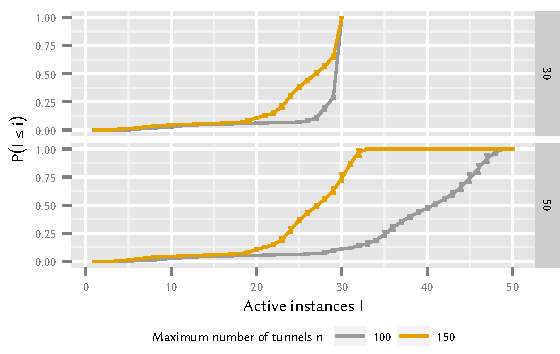
\includegraphics{cloud/virtualized_network_functions/performance_evaluation/figures/instanceuse_multiserver}
  \caption{Impact of the maximum number of tunnels \(n\) and number of servers \maxServers on number of active servers in the virtual \headershortacr{GGSN} model.}
  \label{fig:cloud:virtualized_network_functions:performance_evaluation:virtual_ggsn:instanceuse_multiserver}
\end{figure}

In \reffig{fig:cloud:virtualized_network_functions:performance_evaluation:virtual_ggsn:instanceuse_multiserver} the \gls{CDF} of the number of active servers for four different virtual \gls{GGSN} configurations is displayed.
We study the behaviour of a virtual \gls{GGSN} with \(\maxServers = 30\) servers, where each server can support \(n = 100\) or \(n = 150\) tunnels.
Then, we compare this with a virtual \gls{GGSN} with \(\maxServers = 50\) servers and again \(n = 75\) or \(n = 150\) tunnels.
We observe that increasing the number of supported tunnels \(n\) per server allows a larger percentage of servers to be shut-down or used for other tasks. This demonstrates the scaling capability of the virtualised model quite well.
Note that both the scenario with \(30\) servers \maxServers and \(150\) maximum tunnels \(n\) per server as well as the scenario with \(60\) servers \maxServers and \(75\) maximum tunnels per server sharing the same maximum amount of tunnels, i.e. \(4500\), being right at the centre of the interesting range of candidates.

\begin{figure}
  \centering
  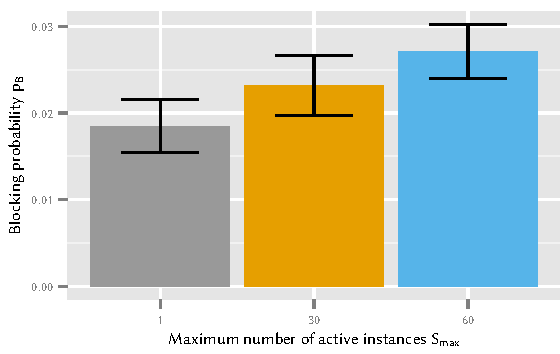
\includegraphics{cloud/virtualized_network_functions/performance_evaluation/figures/blocking_comparison}
  \caption{Impact of blocking probability \blockingprobability on the number of servers compared to the traditional \headershortacr{GGSN}, \(4500\) maximum tunnels per server being on a single server, i.e. \(150\) on \(30\), and \(75\) on \(60\) servers.}
  \label{fig:cloud:virtualized_network_functions:performance_evaluation:virtual_ggsn:blocking_comparison}
\end{figure}

Next, we study the blocking probability of the virtual \gls{GGSN} system in \reffig{fig:cloud:virtualized_network_functions:performance_evaluation:virtual_ggsn:blocking_comparison} and compare it to the results from the traditional \gls{GGSN} model with both systems dimensioned for \(4500\) tunnels.
We observe that, considering the start-up and shut-down time of \SI{300}{\second}, the blocking probability \blockingprobability increases by a factor of \(1.46\) if the virtual \gls{GGSN} is comprised of \(60\) instances \(\maxServers\) dimensioned for \(75\) concurrent tunnels \(n\) , i.e. \(\frac{1}{60}\) of the original server capacity.
In this case \(27\) of all \(60\) servers can be turned off or used for other purposes at \SI{50}{\percent} of the time.
We conclude that choosing more powerful servers decreases the blocking probability but reduces the potential to disable servers.

So far we have considered a conservative start-up and shut-down time of servers \(d\) of 5 minutes, which can potentially occur in non-virtualised available hardware.
In the next section we study the impact of reduced start-up and shut-down times with modern servers with fast storage, e.g. \glspl{SSD}, or containerised applications\footnote{\url{https://www.docker.com/}, \accessed}.

\subsubsection*{Impact of Start-up and Shut-down Times}\label{sec:cloud_virtualized_network_functions:startup_shutdown}

In this section, we first consider the impact of different start-up and shut-down times \(d\) on resource utilisation \(n_A\) and blocking probabilities \blockingprobability.
Afterwards, the influence of varying server start and stop times \(d\) on a fixed combination of maximum tunnels \(n\) and servers \maxServers in the system is examined.

\begin{figure}
  \centering
  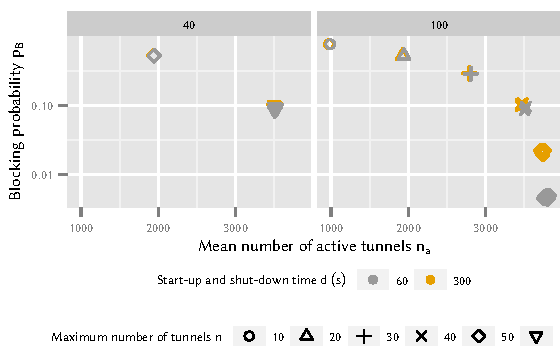
\includegraphics{cloud/virtualized_network_functions/performance_evaluation/figures/compare_util_block}
  \caption{Trade-off between blocking probability \blockingprobability and mean resource utilisation \(n_A\) with regard to maximum number of instances \maxServers, maximum number of tunnels per server \(n\), and start-up and shut-down time \(d\).}
  \label{fig:cloud_virtualized_network_functions:startup_shutdown:compare_util_block}
\end{figure}

\reffig{fig:cloud_virtualized_network_functions:startup_shutdown:compare_util_block} shows scenarios with \(40\) and \(100\) \gls{GGSN} instances \(maxServers\) and  \(1000\) to \(5000\) total concurrent tunnels.
For each scenario, we study the impact of selecting a different maximum number of tunnels \(n\) per server as well as start-up and shut-down times \(d\) on blocking probability \blockingprobability and mean resource utilisation \(n_A\).
The first observation is that by increasing the number of servers \(\maxServers\), i.e. scaling out, the blocking probability \blockingprobability can be decreased, while maintaining a relatively low mean resource utilisation \(n_A\).
In addition to the previous effects, we notice that a higher start-up and shut-down time \(d\) causes a slight increase in blocking probability \blockingprobability for servers with low tunnel capacity \(n\).

\begin{figure}
  \centering
  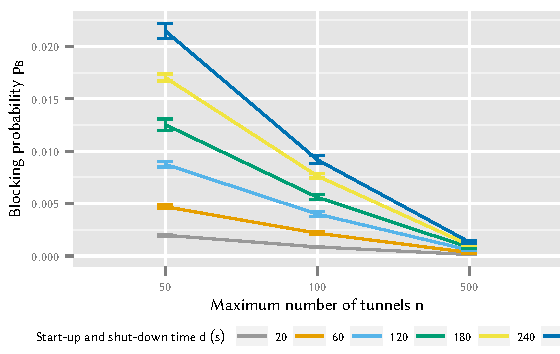
\includegraphics{cloud/virtualized_network_functions/performance_evaluation/figures/compare_maxinstances_block}
  \caption{Influence of start-up and shut-down time \(d\) on blocking probability \(p_B\) with regard to different numbers of supported tunnels per instance \(n\).}
  \label{fig:cloud_virtualized_network_functions:startup_shutdown:compare_maxinstances_block}
\end{figure}

We focus on a specific scenario in \reffig{fig:cloud_virtualized_network_functions:startup_shutdown:compare_maxinstances_block}, where \(5000\) total tunnels should be supported by the system, to study this behaviour in more detail.
To achieve this goal, we consider three types of instances, with the server capacity \(n\) varying between \(50\) and \(500\).
In each case we change the start-up and shut-down time \(d\) between \(20\) and \(\SI{300}{\second}\).
We observe that lower server capacities \(n\) combined with higher start-up and shut-down times \(d\) increase the blocking probability \blockingprobability.
This is due to the server start-up threshold mechanism, used in the model, not taking the additional capacity gained by activating an additional server into account.
If a low capacity server with a long boot time is activated, there is a high probability that the system will quickly expend its capacity again.

Thus, it can be concluded that if smaller instances are to be used, e.g. due to the fact that they are cheaper than large instances, start-up and shut-down times should be kept minimal, for example by using containers or \glspl{SSD}.
